\section{Ouroboros}
Ouroboros~\cite{kiayias2017ouroboros}和Ouroboros-BFT不同,是一种较为基础的基于POS共识的算法。

知乎专栏\footnote{https://zhuanlan.zhihu.com/p/33824015}中对Ouroboros的流程有详细介绍。然而,该论文的主要亮点在于严谨的学术性,以及在顶级密码学期刊发表。在共识层面上能给我们提供的启示非常有限。

\begin{itemize}
	\item 和Ouroboros-BFT一样,时间被分为若干slot。
	\item 若干个连续的slot称作一个朝代(epoch),每个朝代的初始区块(genesis block)记录了所有用户的财富,以及生成一个随机种子。
	\item 每个slot根据随机种子以及记录的财富随机选取出块者。出块者被选取的概率等于其财富的比例。(此处根据随机种子,通过多轮掷硬币函数达成目标)
	\item 每个用户根据最长链原则更新本地存储的区块链。若长时间没收到某个slot的出块信息则认为这个slot的块被废弃。
\end{itemize}
\reffig{fig:Ouroboros2}简要介绍了Ouroboros的流程。文章之后的篇幅大部分用于证明安全性以及探讨分叉的概率。其主结论为一个长为$n$的分叉出现的概率以$2^{-\Omega(\sqrt{n})}$指数级递减。这里不详细介绍。
\begin{figure}
	\centering
	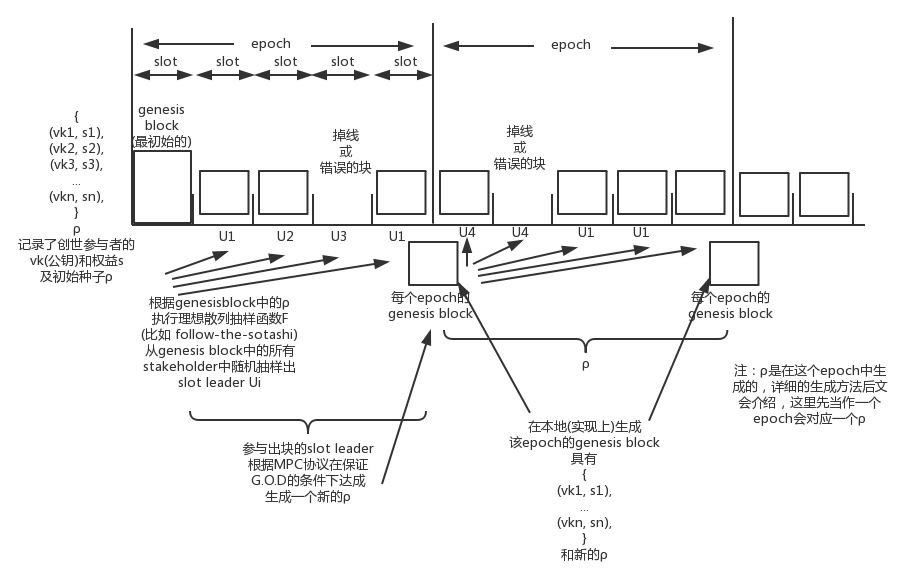
\includegraphics[width=1\textwidth]{../common/Ouroboros.png}
	\caption{Ouroboros简图} 
	\label{fig:Ouroboros2}
\end{figure}
\subsection{思考}
Ouroboros主要亮点在于密码学方面的贡献,在共识层面仅仅是简单的引入POS。在我们看来在permissionless环境的实际应用仍然受限。
\begin{itemize}
	\item 全局时钟的假设仍过强。
	\item 区块没有最终一致性(finality),仅仅为概率一致性。
	\item 对于给定出块者处于超时和给出区块的临界情况的处理未详细介绍。
\end{itemize}
	